%!TEX root = Manuscript.tex


\chapter{Model, Problems}
\label{chap:model}
\minitoc
The model and the proofs presented in this chapter has been introduced in~\cite{DBLP:conf/ict/BarthGLMS18} and extended in a long version of the paper in~\cite{DBLP:journals/corr/abs-1801-07029}.
\section{Model}


Let $[n]$ denote the interval of $n$ integers $\{0,\dots,n-1\}$.


	\subsection{Routes and Contention Points}

  	We study a communication network with pairs of source (s) target (t) nodes between which messages are sent periodically. The routing between each pair of such nodes is given: a \textbf{route} is a sequence of vertices $(s, c_1, \ldots, c_l, t)$. A vertex appears only once in a route. Each vertex $c_i$ corresponds to a contention point, that is the beginning of a link of the communication network shared by several routes. Hence, all vertex appears in several routes, except the first ($s$) and last ($t$) vertex of a route, which are exclusive to the route and represent the source and the target of the message. When modeling a C-RAN network, the first vertex represents the RRH sending of the message by the RRH and the last vertex represents the the same RRH taht receives the answer. 

  	The set of routes is denoted by ${\cal R}$. A route is interpreted as a directed path in a directed multigraph constituted of all routes, where the sets of arcs of the routes are disjoint. The routes contain no loop nor cycle, since all vertices of a route are different. Thus, the directed multigraph is acyclic. An arc in the multigraph may represent several physical links or nodes of the modeled network, which do not induce contention points. 


  	Each arc $(u,v)$ of a route $r$ is labeled by an integer weight $\omega(r,u)$. It represents the time elapsed between the sending of the message of the route $r$ in $u$ and its reception in $v$.
    The {\bf weight of a vertex} $u_i$ in a route $r=(u_0,\dots,u_l)$ is defined by $\lambda(r,u_i)= \sum\limits_{0 \leq j <i} \omega(r,u_j)$. It is the time needed by a message to go from the first vertex of the route to $u_i$. The \textbf{length} of the route $r$ is defined by $\lambda(r)= \lambda(r,u_l)$. 

  	On each route, we can buffer the message only in the BBU. Since the BBU does not correspond to a contention point, we identify the BBU with the next contention point in the route. The set of these contention points with possible buffering is denoted by ${\cal B}$. Each route have thus only one vertex in ${\cal B}$.
  	A \textbf{routed network}, which models the telecommunication network, is a triple $N = (\cal{R},\,\cal{B},\,\omega)$, see Figure~\ref{fig:graphmodel} for an example. 



\begin{figure}
\centering

	
	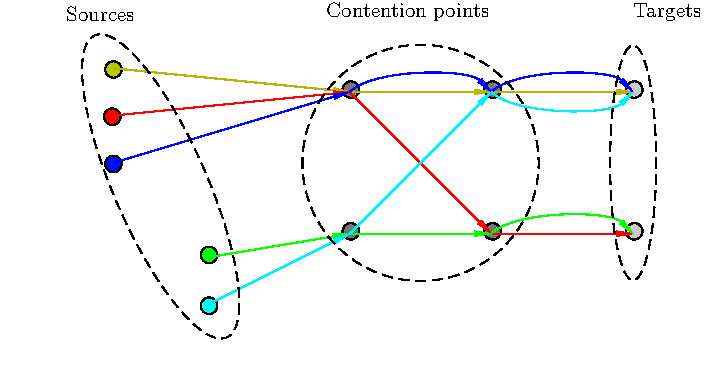
\includegraphics[scale=0.7]{Chapitre3/graphmodel}\\

\caption{A routed network, each route is represented by a colored path}
\label{fig:graphmodel}
\end{figure} 
 

	 
	 
 	\subsection{Dynamic of Datagrams Transmissions}
	    
 		In this thesis, we consider a discretized time. The unit of time is called a {\bf tic}. This is the time needed to send an atomic data in a link of the network. We assume that the speed of the links is the same over all the network. We are developing a prototype of this work based on ethernet base-X~\cite{ieee_8023}, detailled in chapter~\ref{chap:TSN} using standard values for the parameters of the network: the size of an atomic data is $64$ bits, the speed of the links is $10$Gbps, and the length of a tic is thus about $6.4$ nanoseconds. 

        In the process we study, a message, called a {\bf datagram}, is sent on each route from the source node. The \textbf{size} of a datagram is an integer, denoted by $\tau$, it is the number of tics needed by a node to emit the full datagram through a link.  In this thesis, we assume that $\tau$ is the same for all routes. It is justified by our application to C-RAN, where all source nodes are RRHs sending the same type of message. There is no fragmentation: Once a datagram has been emitted, it cannot be fragmented during its travel in the network. 

        Let $r=(s,\dots,t)$ be a route. In order to avoid contention, it is possible to buffer datagrams in the contention points in $\cal{B}$. An \textbf{assignment} $A$ of a routed network $N = (\cal{R},\,\cal{B},\,\omega)$ is a function which associates to each route $r \in \cal{R}$, the pair of integers $A(r) = (o_r,w_r)$.
        The value $o_r$ is the \textbf{offset}, the time at which the datagram is available in the first vertex of $r$. The value $w_r$ is the \textbf{waiting time}: the datagram is buffered 
        for $w_r$ tics in $c \in \cal{B} \cap r$, the vertex representing the BBU.
    		The \textbf{arrival time} of a datagram in the vertex $u_i$ of $r$, is the first time at which the datagram sent on $r$ reaches $u_i$, and is defined by $t(r,u_i) = \lambda(r,u_i) + o_r $ if 
 		    $i < j$ and $t(r,u_i) = \lambda(r,u_i) + o_r + w_r$ otherwise.

 		 Let $u_l$ be the last vertex of the route $r$, the \textbf{transmission time} of the datagram on 
  		$r$ is denoted by $TR(r,A)$ and is equal to $\lambda(r) + w_r$ or equivalently $t(r,u_l) - o_r$. This is the total time taken by the process we study: the sending of the datagram from the RRH to the BBU and the return of the answer back to the RRH. We can decompose this time into $\lambda(r)$, the \emph{physical latency} of the process and $w_r$, the \emph{logical latency}. 
  		We define the \textbf{transmission time} of an assignment $A$ as the worst transmission time of a route: $TR(A) = \displaystyle \max\limits_{r \in {\cal R}} TR(r,A)$. 
        Figure~\ref{fig:datagramtimeline} represents the different events happening during the lifetime  of a datagram  sent on a route $r$.
  		\begin{figure}
  		 \begin{center}
      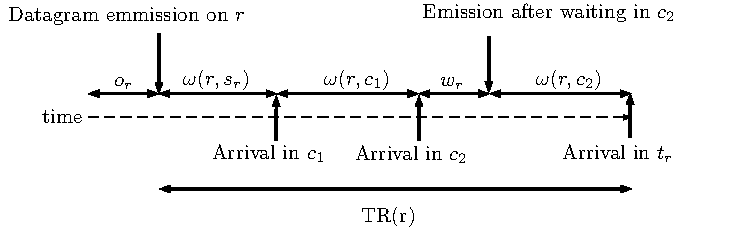
\includegraphics[width=\textwidth]{Chapitre3/time.pdf}
      \end{center}
      \caption{Timeline of a datagram during its travel on a route $r = (s_r,c_1,c_2,t_r)$, with $c_2 \in \cal{B}$}
      \label{fig:datagramtimeline}
  		\end{figure}




 	\subsection{Periodic Emission of Datagrams}

	In the previous section, we have explained how \emph{one} datagram follows its route.
	However, the process we model in this thesis is \emph{periodic}: for each period of $P$ tics, a datagram is sent, from each source node in the network, at its offset. The process is assumed to be infinite, since it must work for an arbitrary number of periods. For a given route, we use the same offset and waiting time in all periods, for simplicity of implementation in real networks and to make our problem more tractable from a theoretical perspective. Hence, at the same time of two different periods, all messages are at the same position in the network: the assignments built are themselves periodic of period $P$. Thus, we only need to consider the behavior of the datagrams on each node of the network during a single period, and to apply the same pattern to every subsequent period. 
 	Using a different offset for each route corresponds to sending their datagram at a different time in the period. This matches our hypothesis that the emissions of the RRHs need not to be synchronized but they share a common global time, useful for coordination of their emission.

 	Let $A$ be an assignment of a routed network $N = (\cal{R},\,\cal{B},\,\omega)$.
    Let us denote by $[r,u]_{P,\tau}$, the set of tics used by a datagram on the route $r$ at vertex $u$ in a period $P$, that is $[r,u]_{P,\tau} = \{t(r,u) + i \mod P \mid 0 \leq i < \tau \}$. This set of tics depends on $A$,
    but $A$ is omited in the notation, since it is always clear from the context.
    Let us consider two routes $r_1$ and $r_2$, they have a {\bf collision} at the contention point $u$ if and only if $[r_1,u]_{P,\tau} \cap [r_2,u]_{P,\tau} \neq \emptyset$.
    The assignment $A$ is said to be \textbf{valid} if, for all contention points $u$ and routes $r_1$ and $r_2$ containing $u$, \emph{$r_1$ and $r_2$ have no collision} at $u$. 
    The validity of an assignment depends on $P$ the period and $\tau$ the size of the messages,
    thus we say that $A$ is a valid \textbf{$(P,\tau)$-assignment}. When $P$ and $\tau$ clear from the context, 
    we denote $[r,u]_{P,\tau}$ by $[r,u]$ and say that $A$ is a valid assignment. 

     The following Figure~\ref{fig:example} illustrates a two valid periodic assignment for different values of $P$ and $\tau$, and the criticity of waiting time in latency reduction. The three routes are depicted by three different colors. If we let $P = 2$ and $\tau = 1$, then there is a $(2,1)$-periodic valid assignment with waiting times zero by taking $0$ as offset for each route. However, for the same routed network but $P=5$ and $\tau = 2$, there is no solution to the problem with waiting times zero. If we allow $1$ tic of waiting time for one route, we can build the valid assignment $((0,0),(2,1),(0,0))$.


  
\begin{figure}[ht]
    \begin{center}
        \scalebox{0.47}{
		\begin{tikzpicture}
\tikzset{
  LabelStyle/.style = { rectangle, rounded corners, draw,
                       font = \bfseries },
  EdgeStyle/.append style = {->} }
  \SetGraphUnit{5}
  \node[draw,circle] (s3) at (4, 2) {$s_2$}; 
  \node[draw,circle] (s2) at (0, 4) {$s_1$}; 
  \node[draw,circle] (s1) at (0, 6) {$s_0$}; 

  \node[draw,circle] (t3) at (14, 7) {$t_2$}; 
  \node[draw,circle] (t2) at (14, 4) {$t_1$}; 
  \node[draw,circle] (t1) at (14, 2) {$t_0$}; 

   \node[circle] (buf) at (10, 6) {$\cal{B}$};
  \SetVertexNoLabel
  \Vertex[x=2,y=5]{A}
    \Vertex[x=10,y=2]{B}
  \Vertex[x=10,y=5]{C}

  \Vertex[x=6,y=3]{E}
     \draw[dashed] (10,3.5) ellipse  (1cm and 2cm);
  \tikzset{
  EdgeStyle/.append style = {green} }
  \Edge[label = 2](s2)(A)

  \Edge[label = 1](A)(C)
 
  \Edge[label = 2](C)(t2)

  
   \tikzset{
  EdgeStyle/.append style = {red} }
  \Edge[label = 2](s3)(E)
  \Edge[label = 2](E)(C)
  \Edge[label = 3](C)(t3) 

     \tikzset{
  EdgeStyle/.append style = {blue} }
  \Edge[label = 1](s1)(A)
  \Edge[label = 2](A)(E)
  \Edge[label = 2](E)(B)
 \Edge[label = 1](B)(t1)

\end{tikzpicture}

}
  	\end{center}
    \caption{A routed network with $(\textcolor{blue}{(0,0)},\textcolor{green}{(0,0)},\textcolor{red}{(0,0)})$ as a $(2,1)$-periodic valid assignment and $(\textcolor{blue}{(0,0)},\textcolor{green}{(2,1)},\textcolor{red}{(0,0)})$ as a $(5,2)$-periodic valid assignment}
    \label{fig:example}
\end{figure}



	\subsection{Periodic Assignment for Low Latency}

      	The period $P$, as well as the size of a message $\tau$ are fixed in our $C-RAN$ settings, but not the buffering policy. Hence, the aim of this section is to find a valid assignment which minimizes the worst latency of the transmissions over the network, that is $TR(A)$. We denote by \mintra the problem of finding the minimal value of $TR(A)$, for a given period, message size and routed network.
      	For simpler hardness proofs and easier reductions, we rather study the decision version of \mintra, that we call \pall for \textbf{P}eriodic \textbf{A}ssignment for \textbf{L}ow \textbf{L}atency. Each route must respect a time limit called a \emph{deadline}. These limits are encoded in a deadline function $d$, which maps to each route $r$ an integer such that $TR(r,A)$ must be less than $d(r)$.
      	We define the \textbf{margin} of a route $r$ in a routed network $N$ with deadline function $d$ as 
        $ d(r) - \lambda(r)$. The margin of a route is the maximum possible waiting time of the route.

     
      \noindent {\bf Periodic Assignment for Low Latency} 

      \noindent {\bf Input:}  A routed network $N$, the integers $P$, $\tau$ and a deadline function $d$.
      
      \noindent {\bf Question:} Does there exist a $(P,\tau)$-periodic assignment of $N$ such that for all $r \in {\cal R}$, $TR(r,A) \leq d(r)$?

	  In the next section, this problem is proved to be $\NP$-hard. In Chapter~\ref{chap:PALL}, we propose heuristics solving the search version of \pall (computing a valid assignment), also denoted by \pall for simplicity. In the definition of \pall, we have chosen to bound the transmission time of each route, in particular we can control the worst case latency. It is justified by our C-RAN application with hard constraints on the latency. 

	 We say that an assignment is \textbf{bufferless} when the waiting time of all routes are zero.
	 The assignment can then be seen as a function from the routes to the integers (the waiting time is omited). We consider a restricted version of \pall, requiring to find a bufferless assignment and studied in Chapter~\ref{chap:PAZL}. This is equivalent to using the deadline function $d(r) = \lambda(r)$, that is the transmission time must be equal to the size of the route, which implies $w_r = 0$ for all $r \in \cal{R}$. This problem is called \textbf{P}eriodic \textbf{A}ssignment for \textbf{Z}ero \textbf{L}atency and is denoted by \pazl. Studying \pazl is simpler: in an instance, there is no need to precise $\cal{B}$ in the routed network nor the deadline function and a solution is just an offset for each route.  Moreover, a solution to \pazl is simpler to implement in real telecommunication networks, since we do not need to deal with any buffering at all.

      An unusual property of assignments is that given a routed network and a deadline, we may have a $(P,\tau)$-periodic assignment but no $(P',\tau)$-periodic assignment with $P' > P$: the existence of an assignment is not monotone with regard to $P$.


	\begin{proposition} \label{prop:monotonic}
	 For any odd $P$, there is a routed network with a $(2,1)$-periodic bufferless assignment but no $(P,1)$-periodic bufferless assignment.
	\end{proposition}

	\begin{proof}
      Let us build $N$, a generalization of the routed network given in Figure~\ref{fig:example}. 
      Let $n$ be an integer, the vertices of the routes are the $v_{i,j}$, $v_i^1$ and $v_i^2$, with $0 \leq i < j <n$. 
      There are $n$ routes denoted by $r_i$, for $i \in [n]$. The route $r_i$ is equal to $(v_i^1,v_{i,1},\dots,v_{i,n-1},v_i^2)$. The weights of the arcs are set so that $\lambda(r_i, v_{i,j}) - \lambda(r_j,v_{i,j})= P$, where $P$ is an odd number smaller than $n$. It is always possible by choosing appropriate values for $\omega(r_i,v_{i,j-1})$ and $\omega(r_j,v_{i-1,j})$. In such a graph, there is no $(P,\tau)$-periodic assignment with zero waiting time, since the problem reduces to finding a $P$-coloring in a complete graph with $n > P$ vertices, the colors being the offsets of the routes.

      If we consider a period of $2$, for all $i \neq j$, $\lambda(r_i, v_{i,j}) - \lambda(r_j, v_{i,j}) \mod 2 = 1$, hence two messages of same offset and size $1$ do not have a collision at $v_{i,j}$. Therefore, the bufferless assignment defined by $A(r_i) = 0$ for all $i \in [n]$ is a valid $(2,1)$-periodic assignment of $N$.      
	\end{proof}


 %    The table of Figure~\ref{tab:summary} summarizes the main notations used in the paper.
 %   \begin{figure}
 %     \begin{center}
 %   \begin{tabularx}{\textwidth}{|c|X|}
 %   \hline
 %    $N = (\cal{R},\,\cal{B},\,\omega)$ & Routed network \\
 %    \hline
 %    $n = |\cal{R}|$ & Number of routes\\
 %    \hline
 %    $P$ & Period\\
 %    \hline
 %    $\tau$ & Size of a message\\
 %    \hline
 %    $\omega(r,u)$ & Weight of the arc $(u,v)$ of $r$ \\
 %    \hline
 %    $\lambda(r,u_i)$ & Length of the route $r$ up to $u_i$\\
 %    \hline
 %    $\lambda(r)$ & Length of the route $r$\\
 %    \hline
 %    $ [t(r,u)]$& Times used in the period by the route $r$ at vertex $v$\\
 %    \hline 
 %    $A$ & Assignment\\
 %    \hline 
 %    $A(r) = (o_r,w_r)$ & Offest and waiting time of the route $r$ given by $A$ \\
 %    \hline 
 %    $TR(A,r)$& Transmission time of the route $r$ for the assignment $A$\\
 %    \hline 
 %    $TR(A)$& Transmission time of the assignment $A$\\
 %    \hline
 %    $d(r)$ & Deadline of the route $r$\\
 %    \hline
 %
 %     \end{tabularx}
 %     \end{center}
 %     \caption{Summary of the notations of the article.}\label{tab:summary}
 %   \end{figure}
  	
  	Let us introduce a few parameters quantifying the complexity of a routed network.
	The \textbf{contention depth} of a routed network is the number of vertices of the longest route of the network minus two. It is the number of contention points on the route with the most vertices on the network, since the first and the last vertex are private to the route. The \textbf{width} of a vertex is the number of routes which contains it. By definition, 
	the first and last vertex of a route are of width $1$, while all other vertices are of width at least $2$
	(otherwise they can be removed).
	The \textbf{contention width} of a routed network is the maximal width of its vertices. 
	Remark that a $(P,\tau)$-periodic assignment of a routed  network must satisfy that $P/\tau$ is larger or equal to the contention width. Now, let us fix $P$ and $\tau$, for a given vertex of contention width $c$, we define its \textbf{load} as $c\tau/P$. It represents the proportion of the period used by datagrams at this contention point. The load of the routed network is the maximum of the loads of its vertices. A routed network must have a load less or equal to one to admit a valid assignment.


 \subsection{The Star Routed Network} \label{sec:star_routed_network}
  
  In this section, we define a family of simple routed networks modeling a Multipoint-to-Multipoint fronthaul (see figure~\ref{fig:star}), which has been designed for C-RAN \cite{tayq2017real}. Let $N = (\cal{R},\,\cal{B},\,\omega)$ be a routed network, we say it is a \textbf{star routed network} if and only if the routes are $\{r_0,\dots,r_{n-1}\}$, $r_i$ is $(s_i,c_1,c_2,t_i)$ and ${\cal B} = \{ c_2 \}$ (datagrams can wait in $c_2$). Star routed networks have contention depth two but a maximal contention width of $n$. The load on each of the two contention points is thus $n\tau / P$.

  The fronthaul network we model with star routed network has a single shared link, which connects all RRHs at one end and all BBUs at the other end. The links are all \emph{full-duplex}, meaning that the datagrams going from RRHs to BBUs do not interact with those going in the other direction. This property does not need to be enforced in our theoritical modeling, but it matches real fronthaul network and we will use such examples for our experiments. 
  The two contention points $c_1$ and $c_2$ model the beginning of the shared link (used to go from the RRHs to the BBUs) and the other end of the shared link (used in the other direction). 
  The computation in the BBU of an answer to a datagram on the route $r$ takes some time.
  In the star routed network, this time is encoded in the weight of the arc between $c_1$ and $c_2$ in $r$. The weight $\omega(r,c_1)$ is the time needed to go through the shared link, then to arrive at the BBU, plus the computation time and the time to return to the shared link, see Figure~\ref{fig:star}.


    Star routed network may seem simplistic, but every network in which all routes share an arc and satisfy a coherent routing condition can be modeled by a star routed network.
    It is common in fronthaul networks, since often all the BBUs are located in the same data-center. In such a situation, we can see the weights of the arcs $(c_1,c_2)$ either as all equals (in that case \pazl is trivial, see Chapter~\ref{chap:PALL}) or different due to the structure of the network inside the data-center and the various hardwares used for the BBUs. 

      
    
  % \begin{minipage}{0.40\linewidth}
    % \includegraphics[scale=0.5]{starfronthaul}\\
      


 %  \end{minipage}\hfill
%\begin{minipage}{0.55\linewidth}   

\begin{figure}
\begin{center}
\scalebox{0.4}{

\begin{tikzpicture}
  \SetGraphUnit{5}
    \tikzset{
  EdgeStyle/.append style = {->} }
   \tikzstyle{VertexStyle}=[shape = circle, draw, minimum size = 30pt]
 

  \node (s1) at (0,4) {
\includegraphics[width = 1cm]{rrh.png}};
  \node[below] at (s1.south) {\huge $r_1$};
  \node (s2) at (0,2) {
\includegraphics[width = 1cm]{rrh.png}};
  \node[below] at (s2.south) {\huge $r_2$};
  \node (s3) at (0,0) {
\includegraphics[width = 1cm]{rrh.png}};
  \node[below] at (s3.south) {\huge $r_3$};
  
   \node (t1) at (12,4) {
\includegraphics[width = 1cm]{bbu.png}};
  \node[below] at (t1.south) {\huge $b_1$};
  \node at (t1.north west) {\textcolor{green}{3}};
  \node (t2) at (12,2) {
\includegraphics[width = 1cm]{bbu.png}};
  \node[below] at (t2.south) {\huge $b_2$};
   \node at (t2.north west) {\textcolor{green}{2}};
  \node (t3) at (12,0) {
\includegraphics[width = 1cm]{bbu.png}};
  \node[below] at (t3.south) {\huge $b_3$};
   \node at (t3.north west) {\textcolor{green}{3}};
    \node (c1) at (4,2) {
\includegraphics[width = 1cm]{switch.png}};
  \node[below] at (c1.south) {\huge $c_1$};
    \node (c2) at (8,2) {
\includegraphics[width = 1cm]{switch.png}};
  \node[below] at (c2.south) {\huge $c_2$};
  
 %\SetVertexNoLabel
  %\Vertex[x=4,y=2]{n1}

  %\Edge[label = $5$](s1)(c1)
  %\Edge[label = $7 + 4+4$](c1)(c2)
  %\Edge[label = $3$](s2)(c1)
   %\Edge[label = $7$](s3)(c1)
  %  \Edge[label = $7+3$](c2)(s2p)
 %  \Edge[label = $7+7$](c2)(s3p)
%\Edge[label = $7 + 5$](c2)(s1p)
\path (s1) edge [<->] node[anchor=south,inner sep = 0.2cm]{$5$} (c1);

\path (s2) edge [<->] node[anchor=south,inner sep = 0.2cm]{$3$} (c1);
\path (s3) edge [<->] node[anchor=south,inner sep = 0.2cm]{$7$} (c1);
\path (c2) edge [<->] node[anchor=south,inner sep = 0.2cm]{$4$} (t2);
\path (c2) edge [<->] node[anchor=south,inner sep = 0.2cm]{$1$} (t3);

\path (c2) edge [<->] node[anchor=south,inner sep = 0.2cm]{$2$} (t1);

\path (c1) edge [<->] node[anchor=south,inner sep = 0.2cm]{$7$} (c2);


  \Vertex[x=14,y=4, L = {\huge $s_1$}]{s1};
  \Vertex[x=14,y=2, L = {\huge $s_2$}]{s2};
\Vertex[x=14,y=0, L = {\huge $s_3$}]{s3};
\Vertex[x=26,y=4, L = {\huge $t_1$}]{s1p};
\Vertex[x=26,y=2, L = {\huge $t_2$}]{s2p};
\Vertex[x=26,y=0, L = {\huge $t_3$}]{s3p};
\Vertex[x=22,y=2, L = {\huge $c_2$}]{c2};

  \Vertex[x=18,y=2, L = {\huge $c_1$}]{c1}
  
 %\SetVertexNoLabel
  %\Vertex[x=4,y=2]{n1}

  %\Edge[label = $5$](s1)(c1)
  %\Edge[label = $7 + 4+4$](c1)(c2)
  %\Edge[label = $3$](s2)(c1)
   %\Edge[label = $7$](s3)(c1)
  %  \Edge[label = $7+3$](c2)(s2p)
 %  \Edge[label = $7+7$](c2)(s3p)
%\Edge[label = $7 + 5$](c2)(s1p)
\path (s1) edge [->] node[anchor=south,inner sep = 0.2cm]{$5$} (c1);

\path (s2) edge [->] node[anchor=south,inner sep = 0.2cm]{$3$} (c1);
\path (s3) edge [->] node[anchor=south,inner sep = 0.2cm]{$7$} (c1);
\path (c2) edge [->] node[anchor=south,inner sep = 0.2cm]{$7+3$} (s2p);
\path (c2) edge [->] node[anchor=south,inner sep = 0.2cm]{$7+7$} (s3p);

\path (c2) edge [->] node[anchor=south,inner sep = 0.2cm]{$7+5$} (s1p);

\path (c1) edge [->] node[anchor=south,inner sep = 0.2cm]{$7+4+\textcolor{green}{2}+4$} (c2);

\path (c1) edge [->,bend left=30] node[anchor=south,inner sep = 0.2cm]{$7+2+\textcolor{green}{3}+2$} (c2);
\path (c1) edge [->,bend right=30] node[anchor=north,inner sep = 0.2cm]{$7+1+\textcolor{green}{3}+1$} (c2);
   \node[circle] (buf) at (22, 0.5) {$\cal{B}$};
   \draw[dashed] (22,2) ellipse  (0.6cm and 1cm);
  %\draw[->,line width=0.5pt] (5,2.51) parabola bend (7.5,3.5) (10,2.51);


\end{tikzpicture}
}



%\end{minipage}

             \caption{Left, a physical fronthaul network and right, the star routed network modeling a round trip in the fronthaul network. The computation time in the BBU is given in green.}

           \label{fig:star}
            \end{center}
           \end{figure}
           
  When solving \pall or \pazl on a star routed network, a period, a datagram size and a deadline function are also given. When the period is fixed, if we can modify the deadline function, we can do several assumptions on the parameters of the star routed network without loss of generality. We say that a star routed network is \textbf{canonical}, for a period $P$, if the weights of the arcs between $c_1$ and $c_2$ are in $[P]$ and the others are equal to zero. Hence, $\lambda(r_i)$, the length of a route is equal to the length of its arc $(c_1,c_2)$. Moreover, $\lambda(r_0) = 0$. See Figure~\ref{fig:canonical} for an example of the canonical star routed network of Figure~\ref{fig:star}.  
  
\begin{figure}
\begin{center}




 \scalebox{0.5}{

\begin{tikzpicture}
  \SetGraphUnit{5}
    \tikzset{
  EdgeStyle/.append style = {->} }
   \tikzstyle{VertexStyle}=[shape = circle, draw, minimum size = 30pt]
   \renewcommand{\VertexLightFillColor}{orange}
  \Vertex[x=0,y=4, L = {\huge $s_1$}]{s1};
  \Vertex[x=0,y=2, L = {\huge $s_2$}]{s2};
\Vertex[x=0,y=0, L = {\huge $s_3$}]{s3};
\Vertex[x=15,y=4, L = {\huge $t_1$}]{s1p};
\Vertex[x=15,y=2, L = {\huge $t_2$}]{s2p};
\Vertex[x=15,y=0, L = {\huge $t_3$}]{s3p};
\Vertex[x=10,y=2, L = {\huge $c_2$}]{c2};

  \Vertex[x=5,y=2, L = {\huge $c_1$}]{c1}
  
 %\SetVertexNoLabel
  %\Vertex[x=4,y=2]{n1}

  %\Edge[label = $5$](s1)(c1)
  %\Edge[label = $7 + 4+4$](c1)(c2)
  %\Edge[label = $3$](s2)(c1)
   %\Edge[label = $7$](s3)(c1)
  %  \Edge[label = $7+3$](c2)(s2p)
 %  \Edge[label = $7+7$](c2)(s3p)
%\Edge[label = $7 + 5$](c2)(s1p)
\path (s1) edge [->] node[anchor=south,inner sep = 0.2cm]{$0$} (c1);

\path (s2) edge [->] node[anchor=south,inner sep = 0.2cm]{$0$} (c1);
\path (s3) edge [->] node[anchor=south,inner sep = 0.2cm]{$0$} (c1);
\path (c2) edge [->] node[anchor=south,inner sep = 0.2cm]{$10$} (s2p);
\path (c2) edge [->] node[anchor=south,inner sep = 0.2cm]{$14$} (s3p);

\path (c2) edge [->] node[anchor=south,inner sep = 0.2cm]{$12$} (s1p);

\path (c1) edge [->] node[anchor=south,inner sep = 0.2cm]{$15$} (c2);

\path (c1) edge [->,bend left=30] node[anchor=south,inner sep = 0.2cm]{$11$} (c2);
\path (c1) edge [->,bend right=30] node[anchor=north,inner sep = 0.2cm]{$9$} (c2);
   \node[circle] (buf) at (10, 0.5) {$\cal{B}$};
   \draw[dashed] (10,2) ellipse  (0.6cm and 1cm);
  %\draw[->,line width=0.5pt] (5,2.51) parabola bend (7.5,3.5) (10,2.51);
 %\draw[->,line width=0.5pt] (5,1.49) parabola bend (7.5,0.5) (10,1.49);
 

\end{tikzpicture}
}

 $d_1 = 25$, $d_2 = 31$, $d_3 = 25$

$\downarrow$


 \scalebox{0.5}{

\begin{tikzpicture}
  \SetGraphUnit{5}
    \tikzset{
  EdgeStyle/.append style = {->} }
   \tikzstyle{VertexStyle}=[shape = circle, draw, minimum size = 30pt]
   \renewcommand{\VertexLightFillColor}{orange}
  \Vertex[x=0,y=4, L = {\huge $s_1$}]{s1};
  \Vertex[x=0,y=2, L = {\huge $s_2$}]{s2};
\Vertex[x=0,y=0, L = {\huge $s_3$}]{s3};
\Vertex[x=15,y=4, L = {\huge $t_1$}]{s1p};
\Vertex[x=15,y=2, L = {\huge $t_2$}]{s2p};
\Vertex[x=15,y=0, L = {\huge $t_3$}]{s3p};
\Vertex[x=10,y=2, L = {\huge $c_2$}]{c2};

  \Vertex[x=5,y=2, L = {\huge $c_1$}]{c1}
  
 %\SetVertexNoLabel
  %\Vertex[x=4,y=2]{n1}

  %\Edge[label = $5$](s1)(c1)
  %\Edge[label = $7 + 4+4$](c1)(c2)
  %\Edge[label = $3$](s2)(c1)
   %\Edge[label = $7$](s3)(c1)
  %  \Edge[label = $7+3$](c2)(s2p)
 %  \Edge[label = $7+7$](c2)(s3p)
%\Edge[label = $7 + 5$](c2)(s1p)
\path (s1) edge [->] node[anchor=south]{$0$} (c1);

\path (s2) edge [->] node[anchor=south,inner sep = 0.2cm]{$0$} (c1);
\path (s3) edge [->] node[anchor=south,inner sep = 0.2cm]{$0$} (c1);
\path (c2) edge [->] node[anchor=south,inner sep = 0.2cm]{$0$} (s2p);
\path (c2) edge [->] node[anchor=south,inner sep = 0.2cm]{$0$} (s3p);

\path (c2) edge [->] node[anchor=south,inner sep = 0.2cm]{$0$} (s1p);

\path (c1) edge [->] node[anchor=south,inner sep = 0.2cm]{$15$} (c2);

\path (c1) edge [->,bend left=30] node[anchor=south,inner sep = 0.2cm]{$11$} (c2);
\path (c1) edge [->,bend right=30] node[anchor=north,inner sep = 0.2cm]{$9$} (c2);
   \node[circle] (buf) at (10, 0.5) {$\cal{B}$};
   \draw[dashed] (10,2) ellipse  (0.6cm and 1cm);
  %\draw[->,line width=0.5pt] (5,2.51) parabola bend (7.5,3.5) (10,2.51);
 %\draw[->,line width=0.5pt] (5,1.49) parabola bend (7.5,0.5) (10,1.49);
 

\end{tikzpicture}
}

 $d_1 = 14$, $d_2 = 21$, $d_3 = 11$

$\downarrow$


 \scalebox{0.5}{

\begin{tikzpicture}
  \SetGraphUnit{5}
    \tikzset{
  EdgeStyle/.append style = {->} }
   \tikzstyle{VertexStyle}=[shape = circle, draw, minimum size = 30pt]
   \renewcommand{\VertexLightFillColor}{orange}
  \Vertex[x=0,y=4, L = {\huge $s_1$}]{s1};
  \Vertex[x=0,y=2, L = {\huge $s_2$}]{s2};
\Vertex[x=0,y=0, L = {\huge $s_3$}]{s3};
\Vertex[x=15,y=4, L = {\huge $t_1$}]{s1p};
\Vertex[x=15,y=2, L = {\huge $t_2$}]{s2p};
\Vertex[x=15,y=0, L = {\huge $t_3$}]{s3p};
\Vertex[x=10,y=2, L = {\huge $c_2$}]{c2};

  \Vertex[x=5,y=2, L = {\huge $c_1$}]{c1}
  
 %\SetVertexNoLabel
  %\Vertex[x=4,y=2]{n1}

  %\Edge[label = $5$](s1)(c1)
  %\Edge[label = $7 + 4+4$](c1)(c2)
  %\Edge[label = $3$](s2)(c1)
   %\Edge[label = $7$](s3)(c1)
  %  \Edge[label = $7+3$](c2)(s2p)
 %  \Edge[label = $7+7$](c2)(s3p)
%\Edge[label = $7 + 5$](c2)(s1p)
\path (s1) edge [->] node[anchor=south]{$0$} (c1);

\path (s2) edge [->] node[anchor=south,inner sep = 0.2cm]{$0$} (c1);
\path (s3) edge [->] node[anchor=south,inner sep = 0.2cm]{$0$} (c1);
\path (c2) edge [->] node[anchor=south,inner sep = 0.2cm]{$0$} (s2p);
\path (c2) edge [->] node[anchor=south,inner sep = 0.2cm]{$0$} (s3p);

\path (c2) edge [->] node[anchor=south,inner sep = 0.2cm]{$0$} (s1p);

\path (c1) edge [->] node[anchor=south,inner sep = 0.2cm]{$0$} (c2);

\path (c1) edge [->,bend left=30] node[anchor=south,inner sep = 0.2cm]{$1$} (c2);
\path (c1) edge [->,bend right=30] node[anchor=north,inner sep = 0.2cm]{$4$} (c2);
   \node[circle] (buf) at (10, 0.5) {$\cal{B}$};
   \draw[dashed] (10,2) ellipse  (0.6cm and 1cm);
  %\draw[->,line width=0.5pt] (5,2.51) parabola bend (7.5,3.5) (10,2.51);
 %\draw[->,line width=0.5pt] (5,1.49) parabola bend (7.5,0.5) (10,1.49);
 

\end{tikzpicture}
}

 $d_1 = 4$, $d_2 = 6$, $d_3 = 6$
 
\end{center}

\caption{Transformation of the star routed network of Figure~\ref{fig:star} to its canonical form, initially with $\tau = 1$, $P=5$, $d_1 = 30$, $d_2 = 34$, $d_3 = 32$.}
\label{fig:canonical}
\end{figure}

  \begin{proposition}\label{prop:canonical}
   Let $I = (N, P, \tau , d)$, with $N = (\cal{R},\,\cal{B},\,\omega)$ a star routed network, then there is 
   $I' = (N', P, \tau , d')$, with  $N' = (\cal{R},\,\cal{B},\,\omega')$ a canonical star routed network, such that:
     $$I \in \pall \Leftrightarrow I' \in \pall \text{ and } I \in \pazl \Leftrightarrow I' \in \pazl$$
  \end{proposition}

  \begin{proof}
  Let us define $\omega'$ and $d'$ from $\omega$ and $d$ in such a way that there is a bijection 
   between valid assignments of $I$ and $I'$, which proves the proposition. In this bijection,
   the offsets $o_i$ for an assignment of $I$ will be mapped to $o'_i$, while the waiting times remain the same.
  
  The routed network $N'$ is equal to $N$ except for the weight function $\omega'$.
  We set the weights of the arcs $(s_i,c_1)$ to zero in $N'$. We obtain the bijection between valid assigments of $I$ and $I'$ by setting $o_i' + \omega(r_i,s_i) = o_i $ and $d'(r_i) = d(i) - \omega(r_i,s_i)$. The weights $\omega'(r_i,c_2)$ are also set to $0$, it does not change the possible collisions
  for an assignment but it changes the transmission time, hence we set $d'(r_i) = d'(r_i) - \omega(r_i,c_2)$
  to preserve the bijection between assignments of $I$ and $I'$. 

  We let $\omega'(r_i,c_1) = \omega(r_i,c_1) \mod P$. Again, it does not change the collisions since computing a possible collision is done modulo $P$. However, we must change $d'$ to be $d'(r_i) = d'(r_i) - \omega(r_i,c_1) + \omega'(r_i,c_1)$.

  Finally, we assume w.l.o.g. that $\omega'(r_0,c_1)$ is the smallest weight among the weights of the arcs
  $(c_1,c_2)$. We let $\omega'(r_i,c_1) = \omega'(r_i,c_1) - \omega'(r_0,c_1)$, which implies that $\omega'(r_0,c_1) = 0$.  All lengths between $c_1$ and $c_2$ change by the same value, hence collisions are not modified. We change $d'(r_i)$ to  $d'(r_i) - \omega'(r_0,c_1)$ for all $i$ so that the constraint on the deadline stay the same.
  \end{proof}

   From now on, we may assume that a star routed network is canonical, using Proposition~\ref{prop:canonical}. To give a instance of \pall where the routed network is a canonical star routed network, it is enough to give the weights of the arcs $(c_1,c_2)$ for all routes, the period, the datagram size, and $d$ the deadline function. 

   Chapter~\ref{chap:PAZL} focuses on solving \pazl on star routed network. Chapter~\ref{chap:PALL} will focus on solving \pall on such topologies.



\section{Hardness of \texttt{PALL} and \texttt{PAZL}}
  \label{sec:complexity}


	We show in this section that \pall is $\NP$-hard by proving $\NP$-hardness for a restricted version: \pazl with $\tau = 1$. We give two proofs that \pazl is $\NP$-complete.
	The first proof works even for contention depth two, but not for star routed networks.
	 For contention depth one, the problem is trivial: either the load is less than one and there is a valid assignment with zero waiting time or there is no valid assignment. 
	 The second proof works for graphs with contention width $2$: the conflicts are locally very simple, but the problem is complex globally nonetheless. Since solving \pall is trivial on trees, it may be interesting to study its complexity on bounded treewidth (or dagwidth) networks, a common property of real networks~\cite{de2011treewidth}.
 

 \begin{theorem}\label{th:hardness_contention_depth}
\pazl is $\NP$-complete on the class of routed networks with contention depth 2.
\end{theorem}
 \begin{proof}
 \pazl is in $\NP$ since given an offset for each route in an assignment, it is easy to check whether there are collisions, in linear time in the routed network's size.
 
  Let $H=(V,E)$ be an undirected graph and let $P$ be its maximal degree. We consider the problem to determine whether $H$ is arc-colorable with $P$ or $P+1$ colors. The arc coloring problem is $\NP$-hard~\cite{holyer1981np} and we reduce it to \pazl to prove its $\NP$-hardness. To do that, we define from $H$ a routed network $N = ({\cal R},\, \omega)$ as follows. 

  Let us choose an arbitrary total order $<$ on $V$.
  For each edge $(u,v) \in E$, if $u<v$, there is a route $s_{u,v},u,v,t_{u,v}$ in ${\cal R}$. 
  All these arcs are of weight $0$. Note that, $N$ is of contention depth $2$, as required by the theorem statement. 

  The existence of a $P$-coloring of $H$ is equivalent to the existence of a $(P,1)$-periodic bufferless assignment of $N$. Indeed, a $P$-coloring of $H$ can be seen as a labeling of its edges by the integers in $[P]$. It induces a bijection between $P$-colorings of $H$ and offsets of the routes of ${\cal R}$, which represent the edges of $H$. Having no collision on some vertex $v$ implies that all offsets of routes going through $v$ are different, since all arcs are of weigth $0$. Hence, edges of $H$ incident to $v$, colored by the offsets of a valid assignment are all of distinct colors. Therefore we have reduced arc coloring to \pazl by a polynomial time transformation which concludes the proof. 
 \end{proof}
 
 Remark that we have used weigths of zero for all arcs in the proof. It is a further restriction to the 
 class of graphs for which \pazl is $\NP$-hard. We could ask the weights to be strictly positive, another possible restriction which makes more sense in our model, since weights represent the delay of physical links. Then, we can prove $\NP$-completness using the same proof, by setting all weights to the period $P$.

We now give a hardness proof for routed networks with contention width two but large contention depth. Note that a vertex of contention depth one does not induce a collision and can be removed from the routed network without loss of generality. The presented reduction can be used to prove an inapproximability result. Let \minpazl be the following problem: given a routed network and $\tau$, find the minimal period $P$ such that there is a $(P,\tau)$-periodic bufferless assignment (a positive instance of \pazl). 


\begin{theorem}\label{th:inapprox}
If $\P \neq \NP$, the problem \minpazl on the classe of routed networks of contention width two cannot be approximated in polynomial time within a factor $n^{1-o(1)}$ where $n$ is the number of routes.
\end{theorem}

\begin{proof}
 We reduce the problem of finding the minimal vertex coloring of a graph to \minpazl. Let $H = (U,E)$ be a graph, an instance of the problem of finding a minimal vertex coloring.  We define the routed network $N$ from $H$ as in Proposition~\ref{prop:monotonic}.
 
 Let $<$ be an arbitrary total order on $U$. 
 The vertices of $N$ are in the set $\{v_{u,w} \mid (u,w) \in E\} \cup \{u^1, u^2 \mid u \in U\}$. 
 For each vertex $u$ in $H$, there is a route $r_u$ in ${\cal R}$, whose first and last vertices
 are $u^1$ and $u^2$. In between, the route contains all vertices $v_{u,w}$, following the order $<$ on the $w$. The weights of all arcs is zero. By construction, a contention vertex corresponds to an edge and belongs to exactly two routes representing the vertices of the edge, thus $N$ is of contention width $2$. This reduction is illustrated in Figure~\ref{fig:reductionminpazl}.

  The existence of a $P$-coloring of $H$ is equivalent to the existence of a $(P,1)$-periodic assignment of $N$ without waiting time: the offset of a route can be identified with the color of the corresponding vertex. Indeed, since all weigths are zero, the absence of collision at contention point $v_{u,w}$ is equivalent to the fact that the offsets of $r_u$ and $r_w$ are different and reciprocally.

   Therefore, if we can approximate the minimum value of $P$ within some factor such that there is a $(P,1)$-periodic assignment, we could approximate the minimal number of colors needed to color a graph within the same factor. The proof follows from the hardness of approximability of finding a minimal vertex coloring~\cite{zuckerman2006linear}.
\end{proof}

    \begin{figure}[ht]
    \centering
    \scalebox{0.37}{
    \begin{tikzpicture}
    \tikzset{
      LabelStyle/.style = { rectangle, rounded corners, draw,
        font = \bfseries },
    EdgeStyle/.append style = {->} }
      \SetGraphUnit{5}
      
      
      \node[draw,circle] (s3) at (4, 2) {$w^1$}; 
      \node[draw,circle] (s2) at (0, 4) {$v^1$}; 
      \node[draw,circle] (s1) at (0, 6) {$u^1$}; 

      \node[draw,circle] (t3) at (12, 3) {$w^2$}; 
      \node[draw,circle] (t2) at (10, 5) {$v^2$}; 
      \node[draw,circle] (t1) at (10, 2) {$u^2$}; 
      

      \tikzstyle{VertexStyle}=[shape = circle, draw, minimum size = 20pt]
  \tikzset{
   VertexStyle/.append style = {blue} }
  \Vertex[x=-8,y=3]{u}
        \tikzset{
      VertexStyle/.append style = {green} }
    \Vertex[x=-7,y=5]{v}

      \tikzset{
      VertexStyle/.append style = {red} }
    \Vertex[x=-6,y=4]{w}
    \tikzset{
      VertexStyle/.append style = {black} }
      
       
       \SetVertexNoLabel
       \Vertex[x=2,y=5]{A}


       \Vertex[x=6,y=3]{E}

       \tikzset{
       EdgeStyle/.append style = {green} }
       \Edge(s2)(A)
       
      \Edge(A)(t2)
 
       
       \tikzset{
      EdgeStyle/.append style = {red} }
       \Edge(s3)(E)
       \Edge(E)(t3) 
  \tikzset{
       EdgeStyle/.append style = {blue} }
       \Edge(s1)(A)
    
       \Edge(A)(E)
              
       \Edge(E)(t1)
       
  \tikzset{
       EdgeStyle/.append style = {black,-} }

       \Edge(u)(v)
       \Edge(u)(w)
     \node (1) at (-3,4){\Huge $\rightarrow$};
      
     \node (2) at (-7,0){\Huge H};
      \node (3) at (10,0){$\Huge N$};
     \end{tikzpicture}
     }
     \caption{Reduction from k-coloring to \minpazl}
     \label{fig:reductionminpazl}
     \end{figure}

The previous theorem implies that \pazl is $\NP$-complete on the class of routed networks with contention width two. This also underlines the fact that, for general graphs, the best $P$ such that there is a 
$(P,\tau)$-periodic assignment may correspond to a very small load. We can build on the reduction of the previous theorem to prove that \mintra, the problem of minimizing $TR(A)$, is hard to approximate too.

\begin{theorem}
If $\P \neq \NP$, the problem \mintra, on graphs of contention width two, cannot be approximated in polynomial time within a factor $n^{1-o(1)}$ where $n$ is the number of routes.
\end{theorem}

\begin{proof}
We reduce the problem of finding the minimal vertex coloring of a graph to \mintra.
 Let $H = (U,E)$ be a graph, instance of the problem of finding a minimal vertex coloring. 
 We define the routed network $N$ in two steps. 

 Let the elements of $U$ be $u_0,\dots, u_{n-1}$. There are $n$ routes in $N$, denoted by $r_i$ for $i \in [n]$. In their first part, they go from $u_i^0$ to $u_i^1$, through some vertices in $\{v_{i,j,k}\}_{i,j,k \in [n]}$ that we later define. Moreover, $u_i^1 \in \cal{B}$, that is the waiting time is added at $u_i^1$. Assume that $r_i$ has offset $o_i$ and $r_j$ has offset $o_j$ and let us fix the datagram size to $1$ and the period to $n$. If $r_i$ and $r_i$ go through some vertex $v_{i,j,k}$, and  $\lambda(r_i,v_{i,j,k}) = \lambda(r_j,v_{i,j,k}) + k$, then to avoid a collision, the equation $o_i \neq o_j + k \mod n$ must be satisfied. If $r_i$ and $r_j$ go through $v_{i,j,k}$ satisfying the previous constraints for all $k \neq l$, it implies $o_i = o_j + l \mod n$. 
 It is easy to choose the weigths of the two arcs going to $v_{i,j,k}$ to realize the previous condition, whatever the choice of weights of the previous arcs of the routes $r_i$ and $r_j$.

We ensure, using the vertices $v_{i,j,k}$ for $k \neq i-j$,
that $o_{i} = o_{j} + i - j \mod n$. It implies that there is some $o$, such that 
$ o = o_{i} - i \mod n$ for all $i \in [n]$. Now, for each route $r_i$, we set the weight of the
arc going to $v_i^1$, from the last vertex of the form $v_{i,j,k}$ in $r_i$, to be $n-i$.
With this construction, we have ensured, that the datagram of $r_i$ arrives at 
$v_i^1$ at time $o$ modulo $n$, for all $i \in [n]$. 

The second part of the routes, from $v_i^1$ to $v_i^2$ is built exactly as in the proof of Theorem~\ref{th:inapprox}. Hence, the waiting time in the vertices $v_i^1$ plays the exact same role as the offset
in the graph of Theorem~\ref{th:inapprox}: the valid $(n,1)$-assignments are in bijection with colorings of $H$, the waiting times corresponding to the colors.

Finally, set the weights of the last arc going to $v_i^2$, for all $i \in [n]$, such that, for all $i,j \in [n]^2$, $\lambda(r_i) = \lambda(r_j)$.  Since all routes are of the same size, $TR(A)$ is equal to the maximal waiting time of $A$. Hence, the maximum waiting time is equal to the number of different waiting times required to have a valid assignment. A valid $(n,1)$-assignment which minimizes $TR(A)$ is in bijection with a minimal proper coloring of $H$, which proves the theorem.

\end{proof}

	We would like to prove hardness for even more restricted networks, in particular star routed networks.
   The problem \pazl on star routed networks is similar to the minimization of makespan in a two flow-shop with delays (see Section~\ref{sec:wtaheuristic}), a problem known to be $\NP$-complete~\cite{yu2004minimizing}. It suggests that \pazl is $\NP$-complete on star routed network, however we have not been able to prove it yet,  because the makespan cannot easily be encoded in \pazl. If we relax the definition of routed network by allowing loops,  we can model a network with a single half-duplex shared link, that is collisions can happen between datagrams going in both directions. This variant can be shown to be $\NP$-complete by a reduction from the subset sum problem, as it is done for a similar problem of scheduling pair of tasks~\cite{orman1997complexity}.
  